\documentclass[]{article}


\usepackage{booktabs}
\usepackage{hyperref}
\usepackage{graphicx}

\usepackage[margin=2.5cm]{geometry}

\usepackage{amssymb, amsmath}
\title{
	Notes on \texttt{Grimsel\_H}\\
	\large GeneRal Integrated Modeling environment for the Supply of
	Electricity and Low-temperature Heat
}
\author{M. C. Soini}

\begin{document}

\maketitle

\tableofcontents

\section{Introduction}\label{introduction}
 
 

\begin{itemize}
\itemsep1pt\parskip0pt\parsep0pt
\item This document describes
	\begin{enumerate}
		\item an  framework implemented in Python using the Pyomo optimization module \ref{implementation_summary}
		\item a simple national-scale linear dispatch model including Switzerland and its neighboring countries \ref{model-documentation}
	\end{enumerate}
\item Power plants are aggregated by type in each country. The generation of
  variable power is based on fixed historical profiles from historic
  data.
\item The inter-node power exchange between countries is optimized endogenously; however, electric grid constraints within the countries are not implemented (copper plate approximation).
\item Stylized model of hydro power: reservoirs with natural inflow are aggregated in each country, both run-of-river plants and pumped hydro storage (PHS) are a separate power plant types with specific operational constraints.
\item The operation during a single year with hourly resolution is optimized.
\item All over-night investment costs are annualized using an appropriate capital recovery factor.
\item The modelling framework Grimsel is designed in a flexible way such that any time resolution $>1$ hour and any subset of hours (e.g.~week\_id=27) can be chosen as a simple keyword argument for fast model runs during testing and development.
\end{itemize}


\section{Implementation summary}\label{implementation_summary}

The model is based on three classes

\begin{itemize}\itemsep1pt\parskip0pt\parsep0pt
\item ModelBase
\item ModelLoop
\item IO
\end{itemize}

The basic role of each class is described below. This is followed by a
summary of their typical usage when running the model.

In addition to these three classes, tailor-made analysis and plotting
modules allow for an efficient processing of the model results. These
parts of Grimsel are not discussed here.

\subsection{BaseModel}\label{basemodel}

The core model is a class inheriting from pyomo.environ.ConcreteModel.
Main purposes:

\begin{itemize}
\itemsep1pt\parskip0pt\parsep0pt
\item
  definition of the linear problem including all constraints and
  variables.
\item
  selection/creation of subsets of input data (in case we don't want to
  use all nodes, or energy carriers, or use a temporal resolution
  \textgreater{} 1 hour or just a subset of the hours of the year)
\item
  handling of CPLEX solver initialization and solver calls
\item
  various model-related convenience methods for pre-solving and
  infeasibility avoidance (see below)
\end{itemize}

The description of the methods follows below:

\subsubsection{\_\_init\_\_}\label{initux5fux5f}

\_\_init\_\_ calls the \_\_init\_\_ of the pyomo.environ.ConcreteModel
and assigns basic keyword arguments, most importantly the time
resolution nhours, the selection of the nodes slct\_node as well as the
selection of the energy carriers slct\_encar (not relevant so far, since
\emph{EL} only). The output schema name sc\_out is generated from a time stamp unless it is provided in the kwargs.

\subsubsection{build\_model}\label{buildux5fmodel}

This calls all methods relevant for the final definition of the model:

\begin{itemize}
\item
  definition of the list of sets dictionary setlst which holds all model
  sets for convenient access; as an example, the following code snippet
  defines the sets of run-of-river plants ror, as well as the set of all
  power plants:
  \begin{verbatim}
  	
  \end{verbatim}

\item
  mapping of input data to the selected time resolution by averaging of
  the hourly profiles
\item
  calculation of the maximum demand from the demand input profile for
  each node (after averaging to the selected time resolution); this is
  used in some constraints
\item
  definition of all sets, parameters, variables and constraints, which
  are primarily found in the corresponding mixin classes. This just
  follows standard pyomo procedures, facilitated by some convenience
  methods
\item
  initialization of the solver
\end{itemize}

Note that this method can only be called after the definition of the
input dataframes, which is typically taken care of by the IO class.

\subsubsection{switch\_soln\_file}\label{switchux5fsolnux5ffile}

Warmstart and solution files names are alternated to allow to use the
last solution as starting values while avoiding excessive disk space use
(which would be the case if we kept all solution files). This method
returns the variables isolnfile, which alternates between 0 and 1, as
well as the temporary solution file name solnfile, which alternates
between e.g. \textbf{TEMPDIR/manual\_soln\_file\_0.cplex.sol} and
\textbf{TEMPDIR/manual\_soln\_file\_1.cplex.sol}.

\subsubsection{run}\label{run}

This method calls the solve method of the solver object. Upon completion
the warmstart and solution file names are switched using the method
switch\_soln\_file.

\subsubsection{presolve\_fixed\_capacities}\label{presolveux5ffixedux5fcapacities}

Runs the model using fixed power plant capacities (or other variables).
This is to obtain starting conditions which are closer to the expected
solution. Presolve variable values are taken from the schema defined by
the string attribute self.sc\_warmstart. Note that the usefulness of
this approach depends strongly on the specific design of the model
constraints and is currently not being used. (It seemed to be highly
useful when constraints on the hour-to-hour ramping of the electricity
production were in place.)

\subsubsection{fill\_peaker\_plants}\label{fillux5fpeakerux5fplants}

Calculate capacity of expensive peaker plants from power capacity
and demand parameters and set the capacity parameter cap\_pwr\_leg
accordingly. This serves to avoid infeasibilities due to insufficient
installed power plant capacity in case the capacities are fixed.
Infeasibilities would be the case if the the peak (residual) demand is
greater than than the total capacity of the (dispatchable) power plants.

\subsection{ModelLoop}\label{modelloop}

This class is used to manage consecutive model calls while varying
parameters, constraint activations/deactivations, etc. The most
important attributes are described here below, followed by the most
important methods.

\subsubsection{nsteps}\label{nsteps}

The basic layout of the model runs/parameter variations is defined by
the list attribute nsteps, which contains the name of the dimension
name, the number of steps, and the type of range. Examples:

\begin{itemize}
\itemsep1pt\parskip0pt\parsep0pt
\item
  (`swvr', 10, numpy.linspace), energy share of wind solar, 10 steps;
  this is varied between 0 and a maximum value (e.g.~50\%), therefore
  numpy.linspace is used to define the step values.
\item
  (`swco', 3, numpy.arange), cost of CO2 emissions; here, the step value
  are used as keys to get the cost from a dictionary (which is
  convenient if the values of CO2 emission prices are not equally
  spaced); therefore, numpy.arange is used
\item
  (`swcd', 2, numpy.arange), charging only wind/solar yes/no; here, the
  step value is used to switch a constraint on or off; therefore, numpy
  is arange is used (which returns {[}0, 1{]} for np.arange(2)).
\end{itemize}

\subsubsection{df\_def\_loop}\label{dfux5fdefux5floop}

This pandas dataframe attribute holds the definitions of all model runs
for each run\_id.

Based on the nsteps, the dataframe df\_def\_loop is defined. Initially
it contains all combinations of all step values. This can be adjusted
outside the ModelLoop class, according to needs. df\_def\_loop is
indexed with the run\_id and for each run\_id defines all

\begin{itemize}
\itemsep1pt\parskip0pt\parsep0pt
\item
  \textbf{steps} with column name equal the dimension name
\item
  \textbf{step ids} with column name equal the dimension name plus
  suffix \_id
\item
  \textbf{step value} with column name equal the dimension name plus
  suffix \_vl; these are typically strings and defined within the
  run\_id loop
\end{itemize}

\textbf{Example}:

\begin{tabular}{@{}lllllll@{}}
\toprule
run\_id & `swvr' & `swcd' & `swvr\_id' & `swcd\_id' & swvr\_vl' &
swcd\_vl'
\\
\midrule
\textbf{0} & 0 & 0 & 0 & 0 & `0.0\%' & `Chg all'
\\
\textbf{1} & 0.5 & 0 & 1 & 0 & `50.0\%' & `Chg all'
\\
\textbf{2} & 1 & 0 & 2 & 0 & `100.0\%' & `Chg all'
\\
\textbf{3} & 0 & 1 & 0 & 1 & `0.0\%' & `Chg ws'
\\
\textbf{4} & 0.5 & 1 & 1 & 1 & `50.0\%' & `Chg ws'
\\
\textbf{5} & 1 & 1 & 2 & 1 & `100.0\%' & `Chg ws'
\\
\bottomrule
\end{tabular}

\subsubsection{select\_run}\label{selectux5frun}

This method obtains all relevant indices and parameters for a certain
slct\_run\_id. For this purpose the relevant row of the dataframe
df\_def\_loop is selected and converted into a set of convenient
dictionaries.

\subsubsection{Other methods}\label{other-methods}

Other methods deal with def\_loop database table definition and writing,
among some convenience methods not described here.

\subsection{IO}\label{io}

This class handles the data exchange between the model and the database,
i.e.:

\begin{itemize}
\itemsep1pt\parskip0pt\parsep0pt
\item
  reading data from the database and define corresponding dataframe
  attributes of the BaseModel; these tables are written to the output
  database schema in order to preserve a consistent set of model data
\item
  (modified) input data is written to the output database schema; this
  concerns hourly profiles whose time resolution is changed\\
\item
  extraction of results and parameter data from the pyomo objects
\item
  initialization and writing of the output database tables
\end{itemize}

The description of the main attributes and methods follows:

\subsubsection{Lists var\_*, par, dual}\label{lists-varux5f-par-dual}

These define the data to be extracted from the model objects and written
to the database. They are lists of tuples (`object\_name', (`set1',
`set2', \ldots{})):

\begin{verbatim}
var_yr = [
		('erg_yr', ('pp_id', 'ca_id', 'bool_out')),
		('erg_fl_yr', ('pp_id', 'nd_id', 'ca_id', 'sf_id')),
		('pwr_ramp_yr', ('pp_id', 'ca_id')), ...]

\end{verbatim}

The column `bool\_out' shown in the example is a binary index which
encodes whether the corresponding energy value is an outward flow
\emph{from the node's perspective}. E.g.:
\begin{itemize}\itemsep0pt
	\item False: power production from power plants, power discharge from storage
	\item True: exports, storage charging power, demand, imports

\end{itemize}

This is used in the analysis.

\subsubsection{Dictionary
dict\_cross\_table}\label{dictionary-dictux5fcrossux5ftable}

Some model variables are appended to other output tables. This
dictionary defines the cross-table writing as
\{`variable\_or\_parameter\_name': `target\_database\_table'\}.
Examples: * Yearly inter-node transmission is appended to yearly energy
generation; * inter-node transmission per time slot is appended to per
time slot power generation table; * the demand profile parameter is
appended to the time slot power generation table.

\subsubsection{write\_runtime\_tables}\label{writeux5fruntimeux5ftables}

Some input tables depend on model parameters (time resolution). They are
written to the output database schema on runtime.

\subsection{Summary of relationships between the classes
IO/ModelBase/ModelLoop}\label{summary-of-relationships-between-the-classes-iomodelbasemodelloop}

The ModelLoop class provides the most top-level objects of a typical series of model runs. The other two classes are instantiated by it. The ModelBase is lowest level class and is accessed by both IO and ModelLoop. The relations are defined in the table below.

\begin{tabular}{@{}llll@{}}
\toprule
& ModelLoop & IO & ModelBase \\
\midrule
\textbf{ModelLoop} & - & instantiates/has attribute & instantiates/has attribute \\
\textbf{IO} & instantiated by/ is attribute of & - & has attribute \\
\textbf{ModelBase} & instantiated by/ is attribute of & is attribute of & - \\
\bottomrule
\end{tabular}

\subsubsection{Sets}

Power plant subsets are defined in the \verb|def_plant| table.


\subsection{Notes on energy carriers and fuels}

The aim is to provide full support for conversions between arbitrary energy carriers while avoiding the definition of explicit hourly input variables. The approach chosen here is composed as follows:

\begin{itemize}
	\item \textbf{Definition of dedicated fuel types which are associated with certain output energy carriers.} For example, \verb|ca_electricity| might be the electricity generated endogenously while \verb|electricity| might be bought electricity. These must be defined separately.
	\item \textbf{Mapping between energy carriers and the corresponding fuels.} In the input table \verb|def_encar|.
	\item \textbf{The input-output energy carrier set} \verb|pp_ndcaca| which contains all relevant combinations of power plants, nodes, output energy carrier, and input energy carrier.
	\item \textbf{An additional demand-term in the supply constraint} which contains the energy carrier "fuel" demand \verb|self.pwr[sy, pp, ca_out] / self.pp_eff[pp, ca_out]|
	of relevant plants, summed over all power plants which make use of the corresponding energy carrier as an input. Note that the supply constraint is defined for all energy carriers separately.

	
\end{itemize}


\subsubsection{Multiple fuels for a plant}

\subsubsection{Storage and energy carriers}

Storage assets (defined by \verb|set_def_st=1| in the input table \verb|def_plant|) operate on energy carriers exclusively. Their input and output is equal to the carrier defined in input table \verb|plant_encar|. The "fuel" assigned to the plant in \verb|def_plant| is not relevant in the model and only used for table consistency and result analysis.

\subsubsection{Energy carriers are node-based}

The production and consumption of energy carriers is node-based, i.e. there is no explicit way of feeding exclusively the output electricity of a wind park into an electrolyzer in order to produce hydrogen if the same node contains other electricity generators. However, this arrangement could still be realized by defining an extra node containing only the wind park and the electrolyzer, and connecting it to the rest of the system through uni-directional inter-node transmission capacity.

\subsection{Input data structure}\label{input-data-structure}

All input data is read from a schema in the PostgreSQL database. The
schema name is a keyword argument of the IO class (default:
\emph{lp\_input}). The database references graph is shown in figure \ref{input_db_ref}
below. This is followed by the description of the input tables.

\begin{figure}[htbp]
\centering
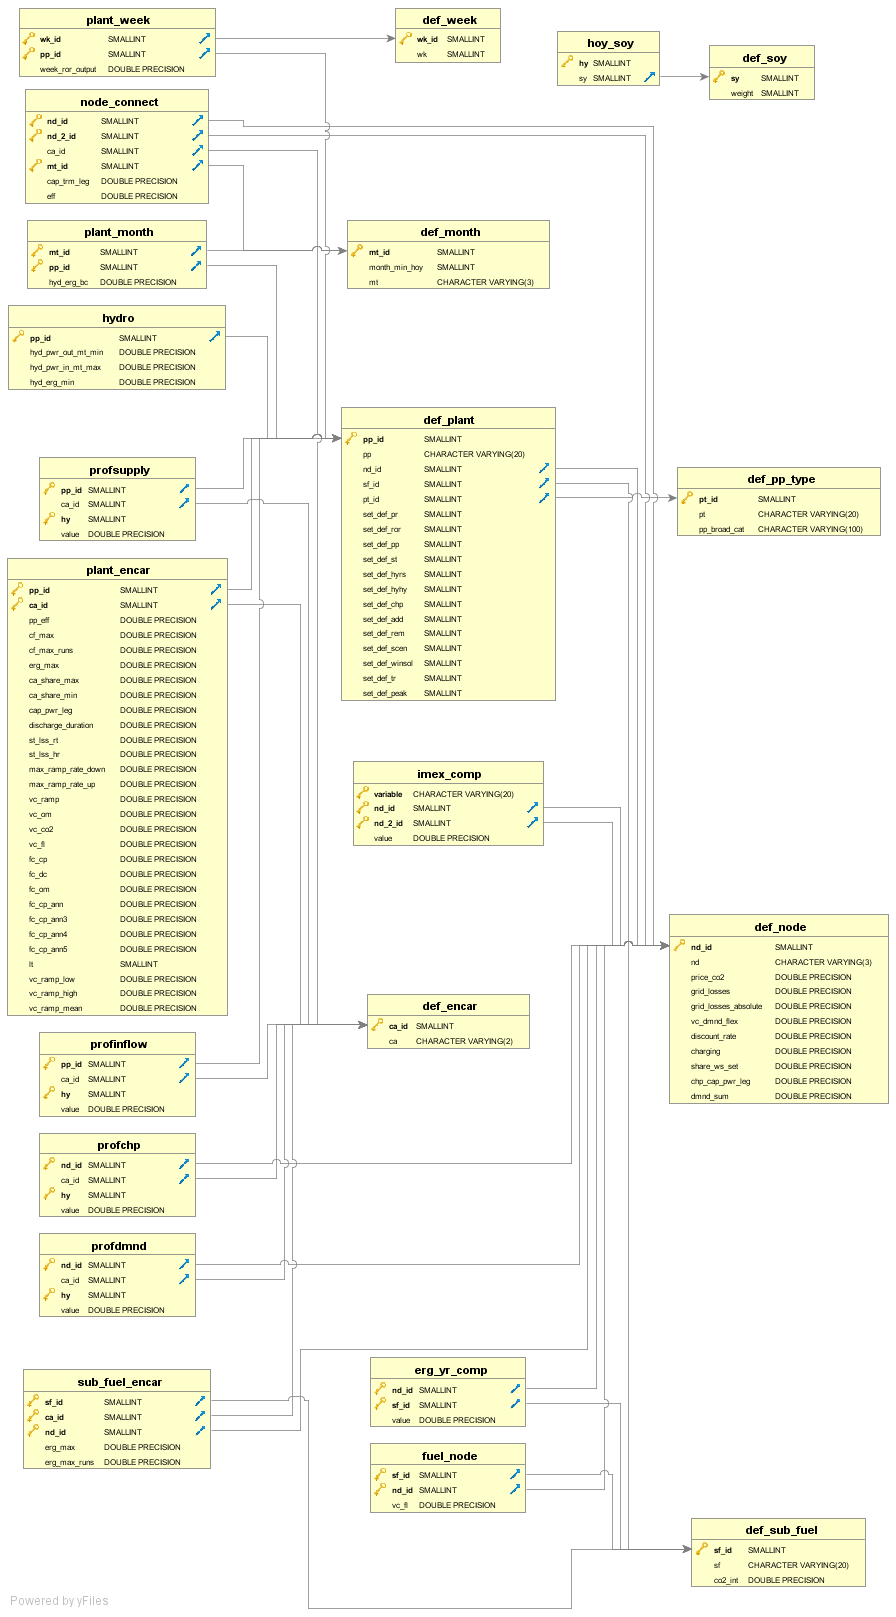
\includegraphics[width=0.7\textwidth]{input_db.png}
\caption{Figure: Input database structure.}
\label{input_db_ref}
\end{figure}

\subsubsection{Description of tables}\label{description-of-tables}

A \emph{consistent} set of these tables in the corrsponding database
schema is strictly required to run the model.

\begin{itemize}
\item
\textbf{def\_encar: Table defining energy carriers.}

\begin{tabular}{@{}llp{10cm}@{}}
\toprule
def\_encar & & \\
\midrule
ca\_id 	& SMALLINT 		& Energy carrier id. \\
ca 		& VARCHAR	 & Energy carrier name. \\
\bottomrule
\end{tabular}

\item \textbf{def\_month: Month definition.}\\
\begin{tabular}{@{}llp{10cm}@{}}
\toprule
def\_month			&			&	\\
\midrule
mt\_id 				& SMALLINT 	& Month id\\
month\_min\_hoy 	& SMALLINT 	& The month's first hour the year. This is used for hydro power filling state boundary conditions. \\
mt & VARCHAR & Month name\\
\bottomrule
\end{tabular}

\item \textbf{def\_node: Table defining nodes (for now: one node per
country).}

\begin{tabular}{@{}llp{10cm}@{}}
\toprule
def\_node & & \\
\midrule
nd\_id & SMALLINT & Node id \{0, 1, 2, 3, 4\} \\
nd & CHARACTER VARYING & Node name \{DE0, AT0, IT0, FR0, CH0\} \\
price\_co2 & DOUBLE PRECISION & Price of $\mathrm{CO_2}$ emissions $[ \mathrm{EUR/t_{CO_2}}]$ \\
grid\_losses & DOUBLE PRECISION & Grid losses as percentage of generation + imports + discharge \\
grid\_losses\_absolute & DOUBLE PRECISION & Absolute grid losses in 2015 for comparison and calibration {[}MWh{]} \\
vc\_dmnd\_flex & 	DOUBLE PRECISION & Cost of flexible additional demand \\
discount\_rate			& DOUBLE PRECISION & Discount rate\\
charging 				& DOUBLE PRECISION & Total charging energy of existing pumped hydro plants, for comparison and calibration. \\
share\_ws\_set 			& DOUBLE PRECISION & Total share of wind and solar. This is currently only used to initialize the corresponding model parameter. \\
chp\_cap\_pwr\_leg 		& DOUBLE PRECISION & Total electric cogeneration capacity. Used in the constraint set\_chp\_cap. \\
dmnd\_sum 				& DOUBLE PRECISION & This is currently used to define the target share of wind and solar.
\\
\bottomrule
\end{tabular}

\item \textbf{def\_plant: Defines power plants}

\begin{tabular}{@{}llp{10cm}@{}}
\toprule
def\_plant & & \\
\midrule
pp\_id & SMALLINT & Power plant id \\
pp & VARCHAR & Power plant name \\
nd\_id & SMALLINT & Node id \\
sf\_id & SMALLINT & Fuel id (one per power plant) \\
pt\_id & SMALLINT & Power plant type id \\
set\_def\_pr & SMALLINT & Yes/No has exogenous profile \\
set\_def\_ror & SMALLINT & Yes/No is run-of-river-plant \\
set\_def\_pp & SMALLINT & Yes/No is dispatchable plant with fuel \\
set\_def\_st & SMALLINT & Yes/No is pure storage plant \\
set\_def\_hyrs & SMALLINT & Yes/No is hydro reservoir plant \\
set\_def\_hyhy & SMALLINT & Yes/No is hybrid reservoir/PHS plant (obsolete) \\
set\_def\_chp & SMALLINT & Yes/No is CHP plant \\
set\_def\_add & SMALLINT & Yes/No capacity can be expanded \\
set\_def\_rem & SMALLINT & Yes/No capacity can be removed \\
set\_def\_scen & SMALLINT & Yes/No is set exogenously by scenarios/parameter variation\\
set\_def\_winsol & SMALLINT & Yes/No is wind or solar plant \\
set\_def\_tr & SMALLINT & Yes/No is transmission (imports or exports) \\
set\_def\_peak & SMALLINT & Yes/No is safety peaker plant (added exogenously to avoid low capacity infeasibilities)\\
\bottomrule
\end{tabular}

\item \textbf{def\_pp\_type: Defines power plant types, which are roughly the same as plant without node-dependence.}

\begin{tabular}{@{}lll@{}}
\toprule
def\_pp\_type & & \\
\midrule
pt\_id & SMALLINT & Power plant type id \\
pt & VARCHAR & Power plant type name \\
pp\_broad\_cat & VARCHAR & Broad power plant category for analysis. \\
\bottomrule
\end{tabular}

\item \textbf{def\_soy: Definition of time slots.}

\begin{tabular}{@{}lll@{}}
\toprule
def\_soy & & \\
\midrule
sy & SMALLINT & Time slot of the year \\
weight & SMALLINT & Number of hours per time slot \\
\bottomrule
\end{tabular}

\item \textbf{def\_sub\_fuel: Defines fuels; called sub-fuel for historic reasons.}

\begin{tabular}{@{}lll@{}}
\toprule
def\_sub\_fuel & & \\
\midrule
sf\_id & SMALLINT & Fuel id \\
sf & VARCHAR(20) & Fuel name \\
co2\_int & DECIMAL & $\mathrm{CO_2}$ emission intensity $[\mathrm{t_{CO_2}/MWh_{fuel}}]$ \\
\bottomrule
\end{tabular}

\item \textbf{def\_week: Week definition. Used for run-of-river operation constraints.}

\begin{tabular}{@{}lll@{}}
\toprule
def\_week & & \\
\midrule
wk\_id & SMALLINT & Month id \\
wk & SMALLINT & Week name (equals wk\_id) \\
\bottomrule
\end{tabular}

\item \textbf{erg\_yr\_comp: Power production stats for comparison.}

\begin{tabular}{@{}lll@{}}
\toprule
erg\_yr\_comp & & \\
\midrule
nd\_id & SMALLINT & Node id \\
sf\_id & SMALLINT & Sub-fuel id \\
value & DOUBLE PRECISION & Yearly electricity generation. \\
\bottomrule
\end{tabular}

\item \textbf{fuel\_node: Defines node-dependent fuel properties.}

\begin{tabular}{@{}llp{10cm}@{}}
\toprule
fuel\_node & & \\
\midrule
sub\_fuel\_id & SMALLINT & Fuel id \\
node\_id & SMALLINT & Node id \\
vc\_fl & DECIMAL & Fuel variable cost $[\mathrm{t_{CO_2}/MWh_{fuel}}]$ (not used in model due to calculation of vc\_fl per MWh\_el in table plant\_encar) \\
\bottomrule
\end{tabular}

\item \textbf{hoy\_soy: Map from hour of the year to time slot of the year;
written during the model initialization.}

\begin{tabular}{@{}lll@{}}
\toprule
hoy\_soy & & \\
\midrule
hy & SMALLINT & Hour of the year \\
sy & SMALLINT & Time slot of the year \\
\bottomrule
\end{tabular}

\item \textbf{hydro: Parameter only relevant for hydro power. This could also
be included in def\_plant or plant\_encar, but is its own table for
convenience.}

\begin{tabular}{@{}llp{10cm}@{}}
\toprule
hydro & &
\\
\midrule
pp\_id & SMALLINT & Power plant id
\\
hyd\_pwr\_out\_mt\_min & DECIMAL & Minimum energy output from hydro
reservoirs during any given month. Expressed as share of maximum monthly
inflow throughout the year.
\\
hyd\_pwr\_in\_mt\_max & DECIMAL & Maximum monthly inflow throughout the
year.
\\
hyd\_erg\_min & DECIMAL & Defines an absolute lower bound for the
monthly production.
\\
\bottomrule
\end{tabular}

\item \textbf{imex\_comp: Import/export statistics for calibration.}

\begin{tabular}{@{}lll@{}}
\toprule
imex\_comp & &
\\
\midrule
variable & VARCHAR & `import'/`export' from nd\_id's perspective
\\
nd\_id & SMALLINT & Node id
\\
nd\_2\_id & SMALLINT & Other node id
\\
value & DOUBLE PRECISION & Yearly electricity {[}MWh{]}
\\
\bottomrule
\end{tabular}

\item \textbf{node\_connect: Defines connections between nodes.}

\begin{tabular}{@{}lll@{}}
\toprule
def\_node\_connect & &
\\
\midrule
nd\_id & SMALLINT & Node id
\\
nd\_2\_id & SMALLINT & The other node id
\\
ca\_id & SMALLINT & Energy carrier transmitted.
\\
mt\_id & SMALLINT & Month id.
\\
cap\_trm\_leg & DECIMAL & Power capacity of connection.
\\
eff & DECIMAL & Efficiency of connection. Set to 99\% for solution
stability.
\\
\bottomrule
\end{tabular}

\item \textbf{plant\_encar: Defines power plant properties depending on
electricity carrier output (would currently not need to be its own table
due to lack of explicit heat production in the model)}

\begin{tabular}{@{}llp{8cm}@{}}
\toprule
plant\_encar & & \\
\midrule
pp\_id & SMALLINT & Power plant id \\
ca\_id & SMALLINT & Energy carrier id \\
pp\_eff & DECIMAL & Power plant efficiency \\
cf\_max & DECIMAL & Maximum capacity factor (availability); during calibration reference year \\
cf\_max\_runs & DECIMAL & Maximum capacity factor (availability); for all other model runs, typical year \\
erg\_max & DOUBLE PRECISION & Maximum yearly power production from this plant (currently not relevant; defined by sub\_fuel in table sub\_fuel\_encar) \\
ca\_share\_max & DECIMAL & maximum share of output energy carrier (currently not relevant) \\
ca\_share\_min & DECIMAL & minimum share of output energy carrier (currently not relevant) \\
cap\_pwr\_leg & DECIMAL & Legacy power capacity \\
discharge\_duration & DECIMAL & Discharge duration for storage and hydro. Serves to calculate the energy capacity from the power capacity. \\
st\_lss\_rt & DECIMAL & Roundtrip losses storage \\
st\_lss\_hr & DECIMAL & Hourly losses storage \\
max\_ramp\_rate\_down & DECIMAL & Maximum ramp rate {[}MW/hour{]} (decrease of power output); currently not used \\
max\_ramp\_rate\_up & DECIMAL & Maximum ramp rate {[}MW/hour{]} (increase of power output); currently not used \\
vc\_ramp & DECIMAL & Cost of ramping {[}EUR/MW{]} \\
vc\_om & DECIMAL & Variable O\&M cost {[}$\mathrm{EUR/MWh_{out}}${]} \\
vc\_co2 & DECIMAL & Variable $\mathrm{CO_2}$ cost $[\mathrm{EUR/MWh_{out}}]$ \\
vc\_fl & DECIMAL & Variable fuel cost $[\mathrm{EUR/MWh_{out}}]$ \\
fc\_cp & DECIMAL & Fixed over-night capital cost $[\mathrm{EUR/MW_{cap}}]$ \\
fc\_dc & DECIMAL & Fixed decommissioning cost (nuclear) $[\mathrm{EUR/MW_{cap}}]$; currently not used \\
fc\_om & DECIMAL & Annual fixed O\&M cost $[\mathrm{EUR/MW_{cap}/yr}]$ \\
fc\_cp\_ann & DECIMAL & Annualized fixed over-night capital cost $[\mathrm{EUR/MW_{cap}/yr}]$ \\
fc\_cp\_ann3 & DECIMAL & Annualized fixed over-night capital cost $[\mathrm{EUR/MW_{cap}/yr}]$ for alternative discount rate \\
fc\_cp\_ann4 & DECIMAL & Annualized fixed over-night capital cost $[\mathrm{EUR/MW_{cap}/yr}]$ for alternative discount rate \\
fc\_cp\_ann5 & DECIMAL & Annualized fixed over-night capital cost $[\mathrm{EUR/MW_{cap}/yr}]$ for alternative discount rate \\
lt & SMALLINT & Life time of power plant {[}$\mathrm{years}${]}. \\
vc\_ramp\_low & DECIMAL & Cost of ramping {[}EUR/MW{]}; alternative values \\
vc\_ramp\_high & DECIMAL & Cost of ramping {[}EUR/MW{]}; alternative values \\
vc\_ramp\_mean & DECIMAL & Cost of ramping {[}EUR/MW{]}; alternative values \\
\bottomrule
\end{tabular}

\item \textbf{plant\_month: Table defining month-dependent power plant
properies.}

\begin{tabular}{@{}lll@{}}
\toprule
plant\_month & & \\
\midrule
mt\_id & SMALLINT & Month id \\
pp\_id & SMALLINT & Plant id \\
hyd\_erg\_bc & DOUBLE PRECISION & Boundary condition hydro reservoir level $[\mathrm{MWh}]$. \\
\bottomrule
\end{tabular}

\item \textbf{plant\_week: Table defining week-dependent power plant
properies.}

\begin{tabular}{@{}lll@{}}
\toprule
plant\_week & & \\
\midrule
wk\_id & SMALLINT & Month id \\
pp\_id & SMALLINT & Plant id \\
week\_ror\_output & DOUBLE PRECISION & Weekly output of run-of-river plants $[\mathrm{MWh}]$.\\
\bottomrule
\end{tabular}

\item \textbf{profchp: Definition of exogenous CHP profile}

\begin{tabular}{@{}lll@{}}
\toprule
profchp & & \\
\midrule
nd\_id & SMALLINT & Node id \\
ca\_id & SMALLINT & Output energy carrier id \\
hy & SMALLINT & Hour of the year \\
value & DOUBLE PRECISION & Hourly capacity factor. \\
\bottomrule
\end{tabular}

\item \textbf{profdmnd: Definition of exogenous demand profile}

\begin{tabular}{@{}llp{10cm}@{}}
\toprule
profdmnd & & \\
\midrule
nd\_id & SMALLINT & Node id \\
ca\_id & SMALLINT & Output energy carrier id \\
hy & SMALLINT & Hour of the year \\
value & DOUBLE PRECISION & Hourly demand $[\mathrm{MW}]$. We choose to define the units as $\mathrm{MW}$ since for time resolution $>1\,\mathrm{hour}$ the profile is averaged over all hours of the time slot. Multiplication with time slot weight happens in the constraint.\\
\bottomrule
\end{tabular}

\item \textbf{profinflow: Definition of exogenous hydro reservoir inflow profile}

\begin{tabular}{@{}llp{10cm}@{}}
\toprule
profinflow & & \\
\midrule
pp\_id & SMALLINT & Power plant id \\
ca\_id & SMALLINT & Output energy carrier id \\
hy & SMALLINT & Hour of the year \\
value & DOUBLE PRECISION & Hourly inflow $[\mathrm{MW}]$. We choose to define the units as $\mathrm{MW}$ since for time resolution $>1\,\mathrm{hour}$ the profile is averaged over all hours of the time slot. Multiplication with time slot weight happens in the constraint. \\
\bottomrule
\end{tabular}

\item \textbf{profsupply: Definition of exogenous wind and solar profiles}

\begin{tabular}{@{}lll@{}}
\toprule
profinflow & & \\
\midrule
pp\_id & SMALLINT & Power plant id \\
ca\_id & SMALLINT & Output energy carrier id \\
hy & SMALLINT & Hour of the year \\
value & DOUBLE PRECISION & Hourly capacity factor. \\
\bottomrule
\end{tabular}

\item \textbf{sub\_fuel\_encar: Parameters depending on input fuel and output energy carrier.} \textbf{\emph{Notes}} * It would be more natural to constrain the fuel availability (erg\_max) through constraints on the input energy. However, the current constraint on the output energy is more straight forward with respect to energy balances.

\begin{tabular}{@{}lll@{}}
\toprule
sub\_fuel\_encar & & \\
\midrule
sf\_id & SMALLINT & Fuel id\\
ca\_id & SMALLINT & Power plant output energy carrier id \\
nd\_id & SMALLINT & Node id \\
erg\_max & DECIMAL & Maximum energy to be produced (calibration). \\
erg\_max\_runs & DECIMAL & Maximum energy to be produced (other model runs). \\
\bottomrule
\end{tabular}

\end{itemize}

\subsection{Output data structure}\label{output-data-structure}

The output schema contains all variables and parameters of the model as well as a copy of the input data.

%
%\section{{[}WORK IN PROGRESS{]}
%Limitations}\label{work-in-progress-limitations}
%
%Discussion of model limitations and their potential implications for the
%model results.
%
%\begin{itemize}
%\itemsep1pt\parskip0pt\parsep0pt
%\item
%  \textbf{Single variable power profiles on the national level}
%\item
%  lower effect of storage due to aggregation of wind/solar profiles;
%  AGORAFLEX2015 discusses smoothening effect when going from pixel to
%  state to country --\textgreater{} implications?
%\item
%  \textbf{Single year optimization}
%\item
%  \textbf{No national grids}
%\item
%  \textbf{Representation of CHP inflexibility}
%\end{itemize}

\section{Model documentation}\label{model-documentation}

\subsection{Supply rule}\label{supply-rule}

The supply constraint makes sure that within each node $n$ and for each
time slot $t$ supply and demand are balanced. Thereby, supply includes
all power generation and storage discharge power $p_{pp,t}$ from all
plants $pp$, as well as imports $\tau^\mathrm{imp}_{\hat n,t}$ from all
neighboring countries $\hat n$. Demand includes the demand profile
$d_{n,t}$, flexible additional demand $d^\mathrm{flx}_{n,t}$ for
curtailments, and charging power $c_{pp,t}$. The supply is reduced by
the transmission and distribution losses $\epsilon$.

\[ \begin{aligned}
&\sum_{pp} p_{pp,t} + \sum_{\hat n}\tau^\mathrm{imp}_{\hat n,t}\\
&=\left(1-\epsilon\right) \left(\sum_{pp} c_{pp,t} + d_{n,t} + d^\mathrm{flx}_{n,t} + \tau^\mathrm{exp}\right) \quad \forall t \in \{0, 1, ..., \bar t\} \quad \forall n \in \{0,1,...,N\}
\end{aligned}
\]

\subsection{Modeling of co-generation}\label{modeling-of-co-generation}

\begin{itemize}
\itemsep1pt\parskip0pt\parsep0pt
\item
  \textbf{Must-run condition based on heat production profile}: The
  output $p_{pp,t}$ from co-generation plants $pp\in C$ (with $C$ the
  set of CHP plants) can be subject to must-run conditions and therefore
  impose inflexibilities on the operation of the power system. Fixed CHP
  profiles $\gamma_{n,t}$ are used to describe the minimum output as a
  fraction of the capacity $P^\mathrm{tot}_{pp}$. See the corresponding
  section for a description of the CHP profile generation. \[
  p_{pp,t} \geqslant \gamma_{n,t} P^\mathrm{tot}_{pp}\quad\forall pp \in C\quad \forall t \in \{0, 1, ..., \bar t\}
  \]
\end{itemize}


\begin{itemize}
\itemsep1pt\parskip0pt\parsep0pt
\item
  \textbf{Investment and retirement:} The total amount of CHP capacity
  (and hence of minimum electricity production from co-generation) must
  not be reduced even if installed capacities can be retired. \[
  \sum_{pp\in C} P^\mathrm{tot}_\mathrm{{pp}} \geqslant P^C_0\quad\forall n \in N
  \]
\end{itemize}

\subsection{Modelling of ramp rate
costs}\label{modelling-of-ramp-rate-costs}

The change of the power output from (thermal) plants leads to a cost
which is modeled as a variable cost on the aggregated absolute changes
of output over the year.

\begin{itemize}
\itemsep1pt\parskip0pt\parsep0pt
\item
  \textbf{Calculation of the ramp rate}: The hourly difference
  $\Delta p_{pp,t}$ in electricity production for each relevant plant
  $pp$ is calculated for each time slot cyclically, i.e.~the last time
  slot $t=\bar t$ loops back to the first $t=0$.
\end{itemize}

\[
\Delta p_{pp,t} = p_{pp,t} - p_{pp,t-1}\quad\forall t\in T,\quad\forall pp\in P
\]

\begin{itemize}
\item
  \textbf{Calculation of the absolute ramp rate}: The absolute ramp rate
  $\left|\Delta p_{pp,t}\right|$ is calculated using the standard linear
  programming approach which makes use of two distinct constraints:
  \[\begin{aligned}
  & \Delta p_{pp,t}\leqslant \left|\Delta p_{pp,t}\right|\\
  \text{and }-&\Delta p_{pp,t}\leqslant \left|\Delta p_{pp,t}\right|
  \end{aligned}\]
\item
  \textbf{Total cost of ramping}: Finally, the total cost of ramping enters the objective function as the sum of all absolute changes in power output $\sum_{pp,t} \left|\Delta p_{pp,t}\right|$ times the corresponding variable cost. Note that here the summation over the time slots does not include a weight factor for the slot length.
\end{itemize}

\subsection{Modelling of hydro power and storage
assets}\label{modelling-of-hydro-power-and-storage-assets}

\subsubsection{Parameters}\label{defining-parameters}

\begin{itemize}
\itemsep1pt\parskip0pt\parsep0pt
\item
  \textbf{Inflow $i_{pp,t}$}: Hourly inflow {[}MW{]} corresponding to
  constant values for all time slots $t$ of each month.
\item
  \textbf{Energy capacities $E^\mathrm{tot} = E^\mathrm{leg}$
  [MWh]}: for hydro plants, the total existing reservoir capacity
  equals the existing (legacy) capacity. Capacity additions and
  retirements are not considered. The same holds for the power
  capacities: $P^\mathrm{tot} = P^\mathrm{leg}$ {[}MW{]}.
\item
  \textbf{Boundary conditions of filling levels $l^\mathrm{bc}_{pp,t}$}
  for time slots $t\in T^\mathrm{bc}_{pp}$ from the corresponding
  sub-set of time slots $T^\mathrm{bc}_{pp}$. (In practice this applies
  to the first time slot of January).
\end{itemize}

\subsubsection{Constraints}\label{constraints}

\begin{itemize}
\item
  \textbf{Reservoir level (reservoirs)} $e_{pp,t}$ in time slot $t$,
  plant $pp$: Filling level during last time slot plus inflow $i_{pp,t}$
  minus electricity production $p_{pp,t}$, times the weight of time
  slots $w_t$ {[}hours{]}. The last time step $t=\bar t$ loops back to
  the first $t=0$, i.e.~time is circular for each year.
  \[ e_{pp,t} = e_{pp,t-1} + (i_{pp,t} - p_{pp,t})\cdot w_t \quad \forall t \in \{0, 1, ..., \bar t\}\]
\item
  \textbf{Reservoir level (Pumped hydro storage) and state of charge
  (SOC, other storage assets)} Pumped hydro storage is modeled like all
  other storage assets. No natural inflow is assumed to be available.
  The total round-trip losses $\epsilon$ are partly attributed to
  charging and discharging.
  \[ e_{pp,t} = e_{pp,t-1} + \left(c_{pp,t}\sqrt{1-\epsilon} - p_{pp,t}/\sqrt{1-\epsilon}\right) \cdot w_t \quad \forall t \in \{0, 1, ..., \bar t\}\]
\item
  \textbf{Boundary conditions} on reservoir levels from reported filling
  levels $l^\mathrm{bc}_{pp}$ during a subset of hours
  $T^\mathrm{bc}_{pp}$. Typically 50\% at the beginning of the year.
  \[ e_{pp,t} = l^\mathrm{bc}_{pp} \quad \forall t \in T^\mathrm{bc}_{pp}\]
\item
  \textbf{Capacity constraints} of power output $p_\mathrm{{pp},t}$,
  charging $c_\mathrm{{pp},t}$ and reservoir filling levels/SOC due to
  limited capacities $E^\mathrm{tot}$ and $P^\mathrm{tot}$:
\end{itemize}

\[\begin{aligned}
&e_\mathrm{{pp},t} \leqslant E^\mathrm{tot}_\mathrm{{pp}}  \quad \forall t \in \{0, 1, ..., \bar t\}\\
&p_\mathrm{{pp},t} \leqslant  P^\mathrm{tot}_\mathrm{{pp}}  \quad \forall t \in \{0, 1, ..., \bar t\}\\
&c_\mathrm{{pp},t} \leqslant  P^\mathrm{tot}_\mathrm{{pp}}  \quad \forall t \in \{0, 1, ..., \bar t\}
\end{aligned}\]

\begin{itemize}
\item
  \textbf{Minimum monthly production of reservoirs}: All monthly
  productions $p_{pp,m} = \sum_{t \in T_{pp,m}} p_{pp,t}$ must be
  greater or equal a certain share $\sigma_{pp}$ of the maximum monthly
  inflow $i_{pp,m,\max} = \max_m \{i_{pp,m}\}$, with the monthly sums
  $i_{pp,m} = \sum_{t \in T_{m}} i_{pp,t}$ of the inflow. $T_{m}$
  denotes the subset of time slots in month $m$. This approximates
  operating constraints due to must-flow conditions.
  \[ p_{pp,m,\min} \leqslant \sigma_{pp}  i_{pp,m,\max}\]
\item
  \textbf{Minimum filling levels of reservoirs}: From the reported data
  on the filling levels in reservoirs it is evident that they never fall
  below a certain minimum (most notably: Italy). A certain minimum is
  defined for each reservoir hydro power plant which decreases the
  effective storage energy capacity.
\end{itemize}

\[e_{pp,t} \geqslant e_{pp,\min}\]

\subsection{Modeling of run-of-river
plants}\label{modeling-of-run-of-river-plants}

\begin{itemize}
\itemsep1pt\parskip0pt\parsep0pt
\item
  \textbf{Weekly power output}: Run-of-river plants
  $pp\in P_\mathrm{ror}$ are a separate class of power plants with
  distinct operation constraints. The weekly production $p_{pp,w}$ must
  add up to the exogenous weekly inflow $i_{pp,w}$: \[
  p_{pp,w} \leqslant i_{pp,w}\quad \forall w\in W,\,pp\in P_\mathrm{ror}
  \]
\item
  \textbf{Must-flow conditions}: Within each week the power plants are
  dispatchable, except for an 80\% base load component which
  approximates the rather restrictive must-flow conditions of this power
  plant class. With the number of hours (weight) $w_w$ of week $w$:
  \[p_{pp,w}\cdot 0.8/w_w \leqslant p_{t,pp}\quad \forall t\in \{0,...,\bar t\}\]
\end{itemize}

\subsection{Short description of objective
function}\label{short-description-of-objective-function}

The objective function to be minimized is the sum over all costs
included in the model:

\begin{itemize}
\itemsep1pt\parskip0pt\parsep0pt
\item
  \textbf{Fuel costs} of each power plant $pp$, proportional to the
  total power plant output $\sum_t p_{pp,t}$
\item
  \textbf{CO${}_2$ emission costs} of each power plant $pp$,
  proportional to the total power plant output $\sum_t p_{pp,t}$; note
  that this does not consider CO${}_2$ emissions due to fuels being
  burned during the off-line phase of the start-up and shutdown process.
\item
  \textbf{Variable operation and maintenance costs} of each power plant
  $pp$, proportional to the total power plant output $\sum_t p_{pp,t}$
\item
  \textbf{Cost of flexible demand} (curtailment) proportional to the
  total sum $\sum_t d^\mathrm{flx}_t$
\item
  \textbf{Ramping costs} for each plant $pp$ proportional to the total
  absolute power output change $\sum_t \left|\Delta p_{pp,t}\right|$
\item
  \textbf{Fixed operation and maintenance costs} for each plant
  proportional to the total installed power capacity
  $\bar p_{pp}^\mathrm{tot}$
\item
  \textbf{Investment costs for new power plant capacity} for each plant,
  proportional to the newly installed power capacity
  $\bar p_{pp}^\mathrm{add}$
\end{itemize}


%\newpage
%\include{data_sources_chapter}

\end{document}
